\begin{table*}[t]
    \setlength{\tabcolsep}{2pt}
    \centering
    \begin{tabular}{cccccccccc} % Add a vertical line to separate the multirow image
        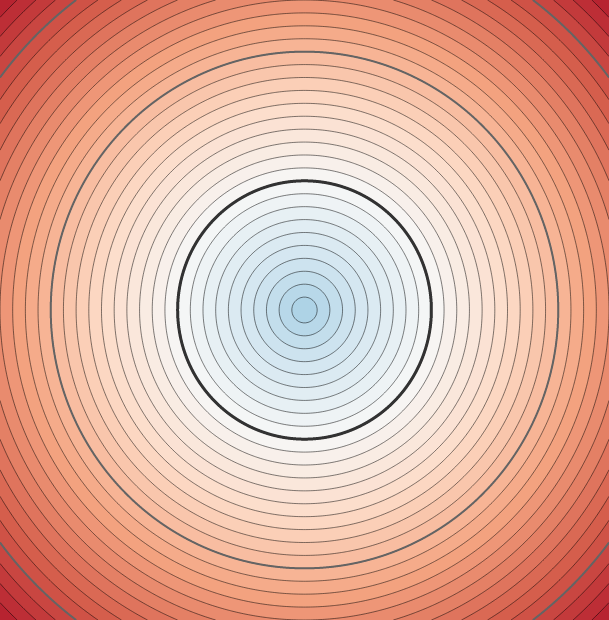
\includegraphics[width=0.09\textwidth]{figures/phase-boundary-exp/2D/circle-gt.png} & 
        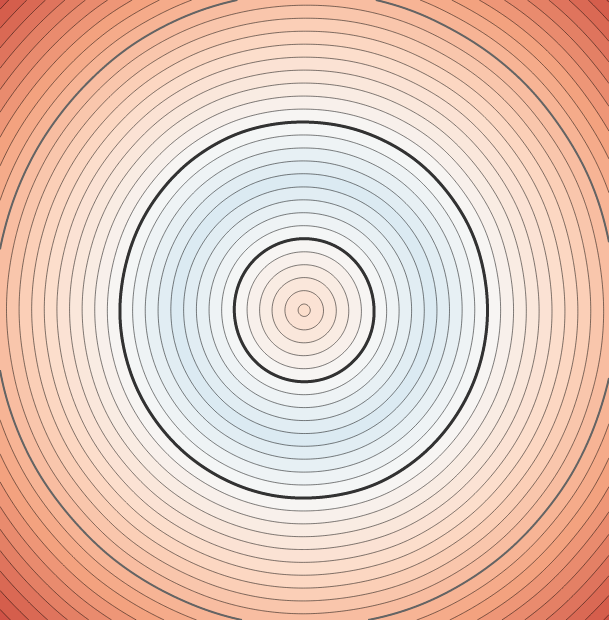
\includegraphics[width=0.09\textwidth]{figures/phase-boundary-exp/2D/circle-0.1.png} & 
        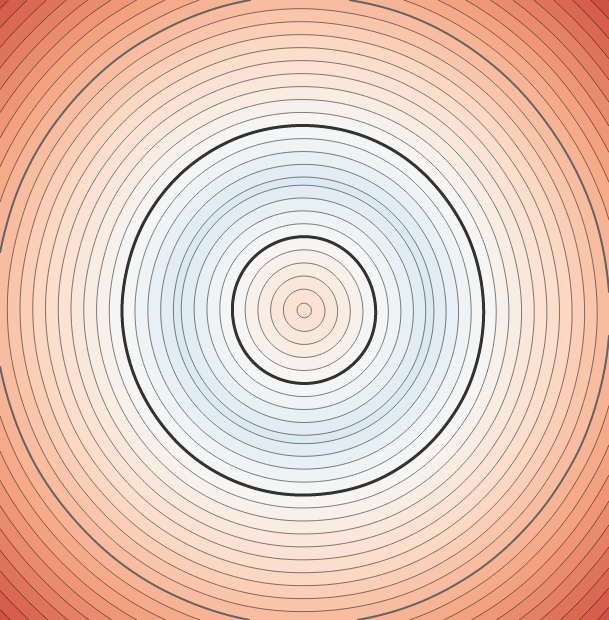
\includegraphics[width=0.09\textwidth]{figures/phase-boundary-exp/2D/circle-0.2.png} & 
        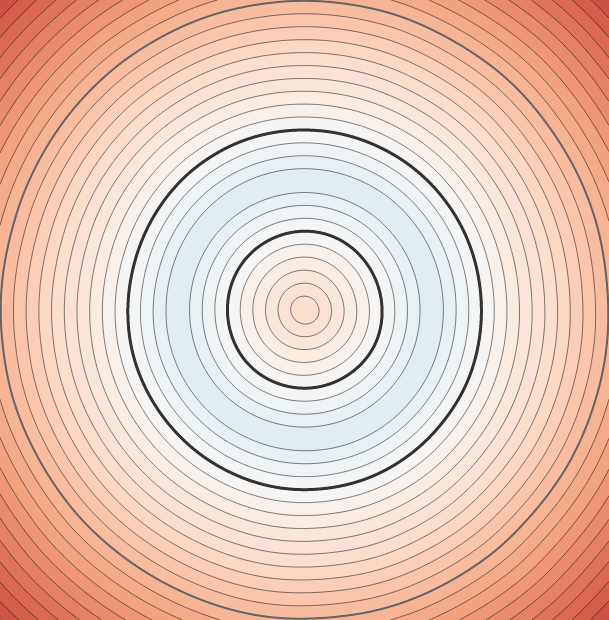
\includegraphics[width=0.09\textwidth]{figures/phase-boundary-exp/2D/circle-0.3.png} & 
        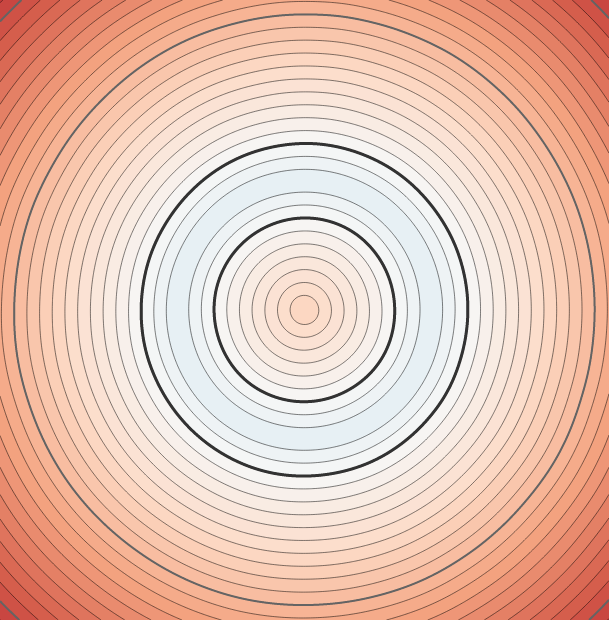
\includegraphics[width=0.09\textwidth]{figures/phase-boundary-exp/2D/circle-0.5.png} &
        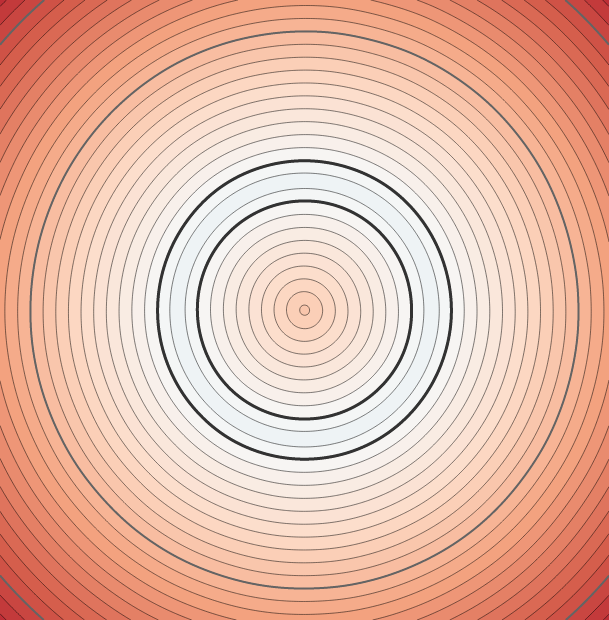
\includegraphics[width=0.09\textwidth]{figures/phase-boundary-exp/2D/circle-1.0.png} & 
        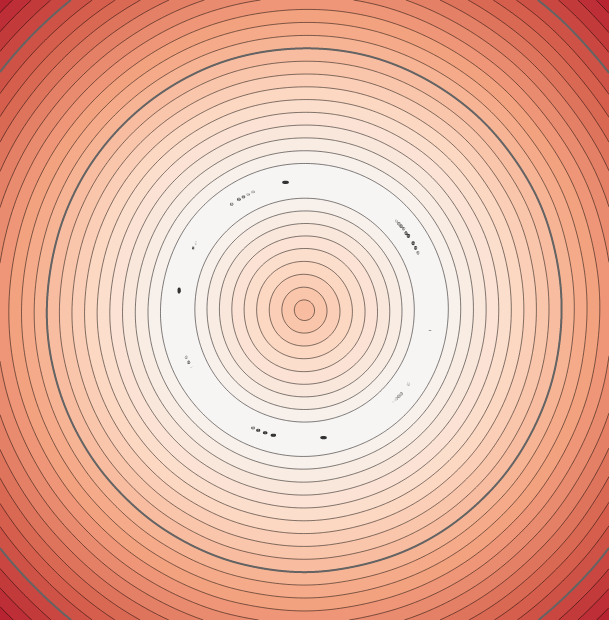
\includegraphics[width=0.09\textwidth]{figures/phase-boundary-exp/2D/circle-2.0.png} & 
        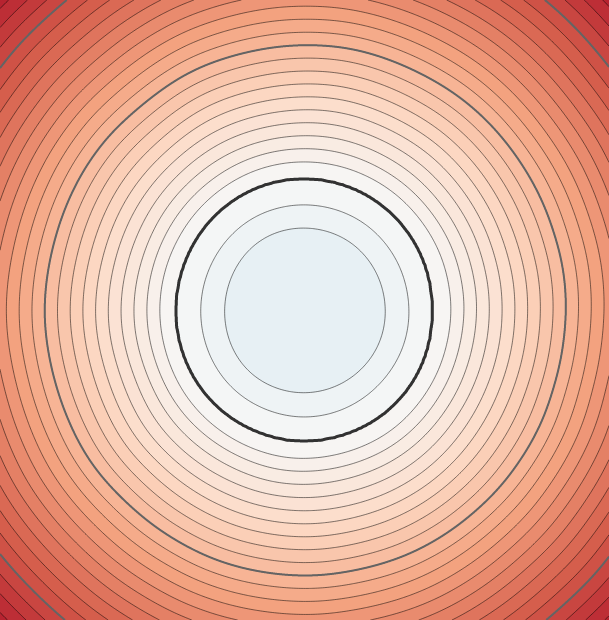
\includegraphics[width=0.09\textwidth]{figures/phase-boundary-exp/2D/circle-5.0.png} & 
        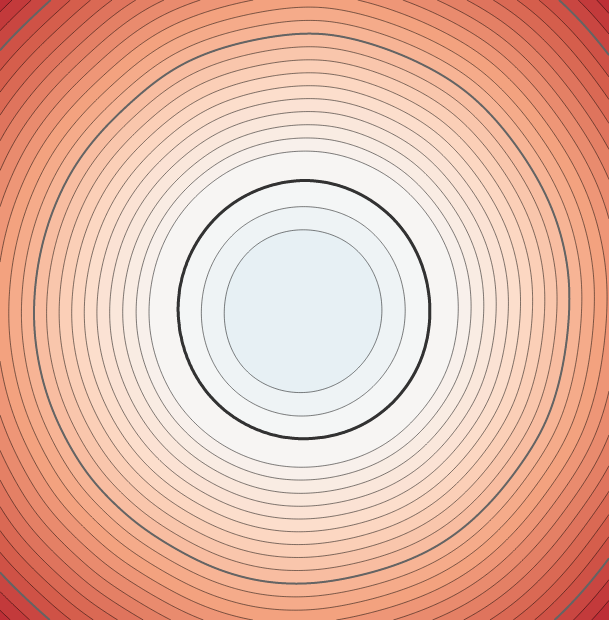
\includegraphics[width=0.09\textwidth]{figures/phase-boundary-exp/2D/circle-10.0.png} & 
        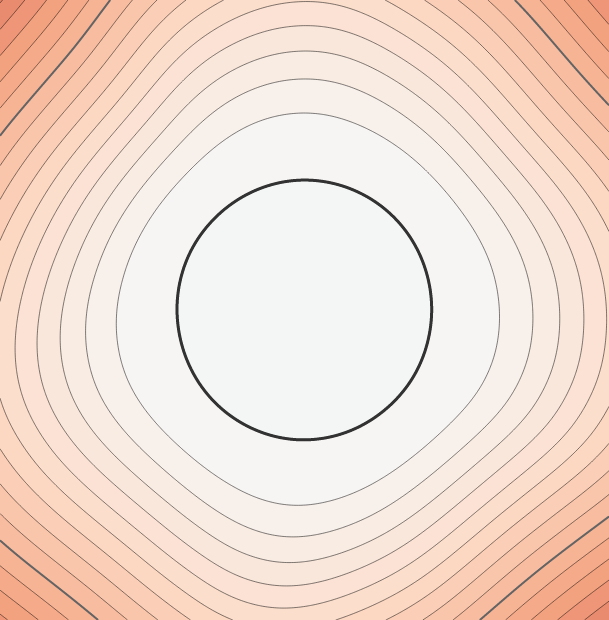
\includegraphics[width=0.09\textwidth]{figures/phase-boundary-exp/2D/circle-20.0.png} \\ [1ex]
        
        GT & $w_b = 0.1$ & $w_b = 0.2$ & $w_b = 0.3$ & $w_b = 0.5$ & $w_b = 1.0$ & $w_b = 2.0$ & $w_b = 5.0$ & $w_b = 10.0$ & $w_b = 20.0$ \\ [1ex]
        \toprule
        IoU & 0.3288 & 0.3330 & 0.3242 & 0.2975 & 0.2138 & 0.0022 & 0.9693 & 0.9912 & 0.9917 \\
        Chamfer & 0.2244 & 0.2138 & 0.1955 & 0.1434 & 0.0777 & 0.0175 & 0.0080 & 0.0026 & 0.0025 \\
        Hausdorff & 0.2315 & 0.2216 & 0.1991 & 0.1455 & 0.0799 & 0.1584 & 0.0150 & 0.0102 & 0.0105 \\
        RMSE & 0.2318 & 0.2209 & 0.2085 & 0.1740 & 0.1477 & 0.1476 & 0.0481 & 0.0681 & 0.3004 \\
        MAE & 0.2237 & 0.2122 & 0.1982 & 0.1552 & 0.1048 & 0.0556 & 0.0336 & 0.0610 & 0.2744 \\
        SMAPE & 0.9159 & 0.8814 & 0.8404 & 0.7059 & 0.5333 & 0.3396 & 0.2028 & 0.3291 & 1.0863 \\
        \bottomrule
    \end{tabular}
    \caption{Comparison of PHASE results on a circle with different $w_b$ values. The color scale is the same as in \Cref{fig:phase-boundary-weight}.}
    \label{fig:phase-boundary-weight-circle}
\end{table*}

\begin{table*}[t]
    \setlength{\tabcolsep}{4pt}
    \centering
    \begin{tabular}{cccccccccc}
        \toprule
        $w_b$ & $0.1$ & $0.2$ & $0.3$ & $0.5$ & $1.0$ & $2.0$ & $5.0$ & $10.0$ & $20.0$ \\
        \midrule
        IoU & 0.2026 & 0.1843 & 0.2050 & 0.2089 & 0.2505 & 0.2061 & 0.3899 & 0.4838 & 0.4696 \\
        Chamfer & 0.2663 & 0.3122 & 0.2504 & 0.1785 & 0.1067 & 0.0499 & 0.0793 & 0.0888 & 0.1030 \\
        Hausdorff & 0.5692 & 0.7001 & 0.5635 & 0.4191 & 0.3446 & 0.3747 & 0.4567 & 0.4383 & 0.5407 \\
        RMSE & 0.4644 & 0.3314 & 0.2382 & 0.1606 & 0.1111 & 0.0734 & 0.0567 & 0.0747 & 0.1282 \\
        MAE & 0.4332 & 0.3114 & 0.2265 & 0.1500 & 0.0918 & 0.0413 & 0.0405 & 0.0623 & 0.1112 \\
        SMAPE & 1.2558 & 1.1504 & 1.0870 & 0.9475 & 0.8107 & 0.5873 & 0.7191 & 0.8877 & 1.1477 \\
        \bottomrule
    \end{tabular}
    \caption{Mean metrics of PHASE results with different $w_b$ values on the full 2D dataset.}
    \label{tab:phase-boundary-weight-metrics}
\end{table*}

\begin{figure*}[t]
    \setlength{\tabcolsep}{1pt}
    \centering
    \begin{tabular}{ccccccccc}
        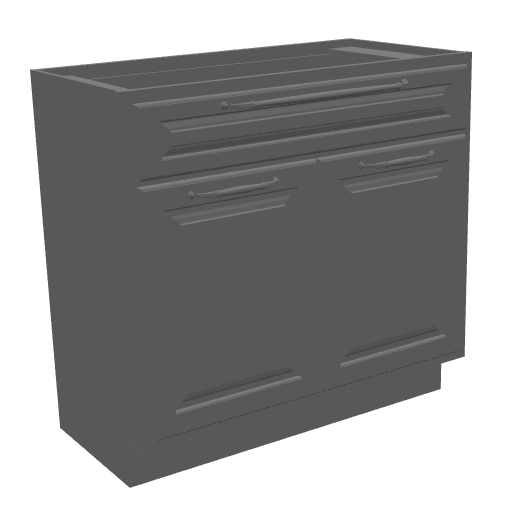
\includegraphics[width=0.11\textwidth]{figures/phase-boundary-exp/3D/cabinet-b0f329dc43af0fbd4da5feafe6f1c8fc-mesh.png} &
        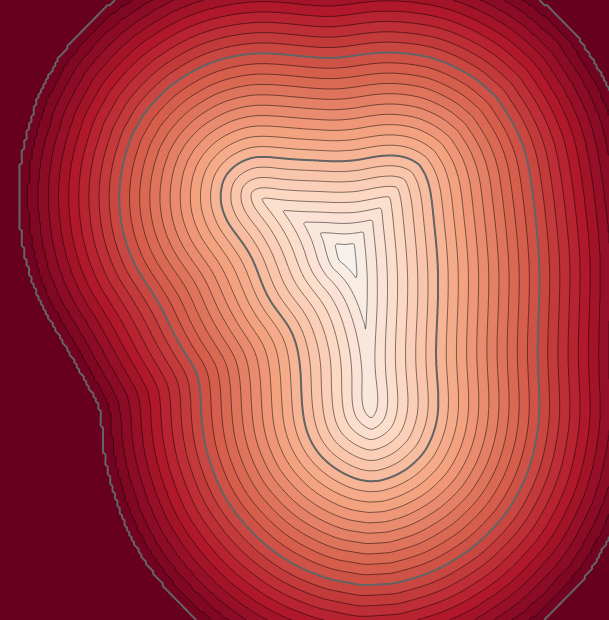
\includegraphics[width=0.11\textwidth]{figures/phase-boundary-exp/3D/cabinet-b0f329dc43af0fbd4da5feafe6f1c8fc-0.1.png} & 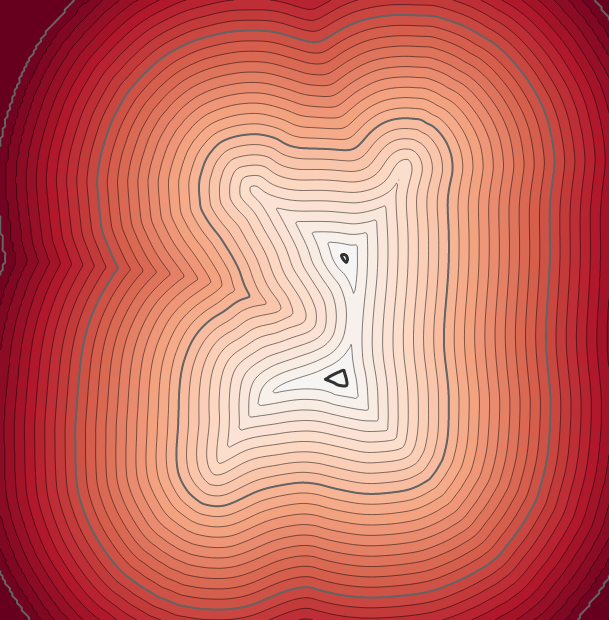
\includegraphics[width=0.11\textwidth]{figures/phase-boundary-exp/3D/cabinet-b0f329dc43af0fbd4da5feafe6f1c8fc-0.2.png} & 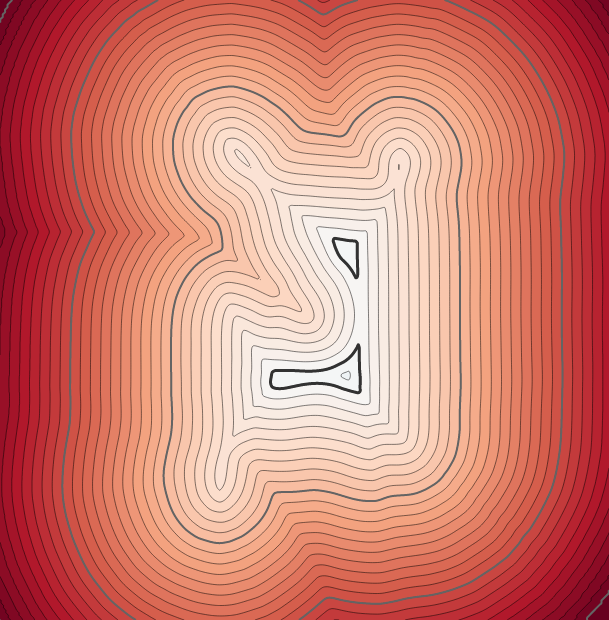
\includegraphics[width=0.11\textwidth]{figures/phase-boundary-exp/3D/cabinet-b0f329dc43af0fbd4da5feafe6f1c8fc-0.3.png} & 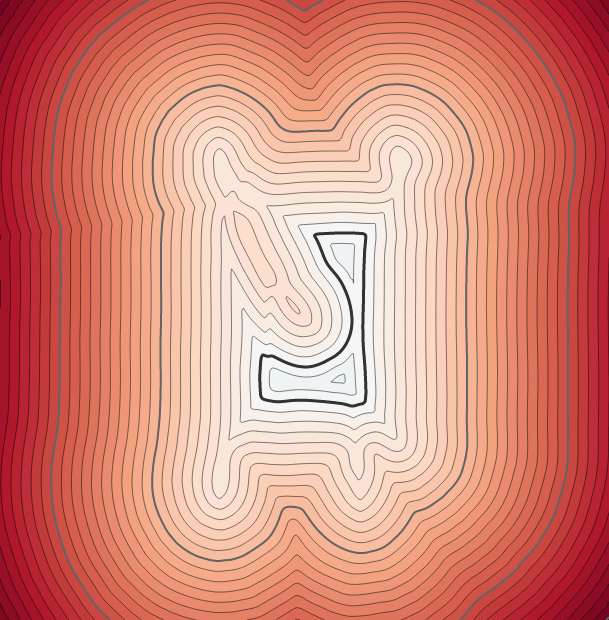
\includegraphics[width=0.11\textwidth]{figures/phase-boundary-exp/3D/cabinet-b0f329dc43af0fbd4da5feafe6f1c8fc-0.5.png} &
        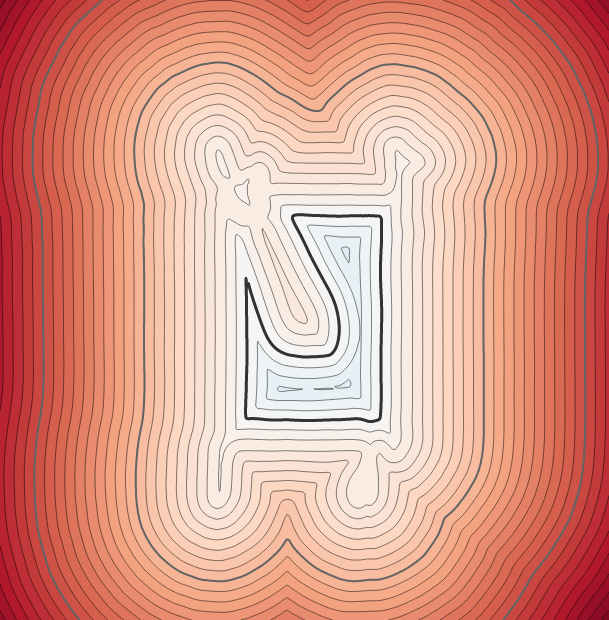
\includegraphics[width=0.11\textwidth]{figures/phase-boundary-exp/3D/cabinet-b0f329dc43af0fbd4da5feafe6f1c8fc-1.0.png} & 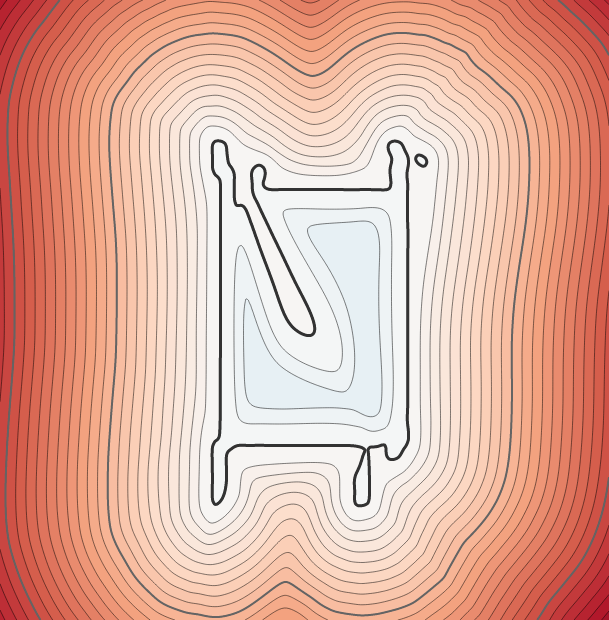
\includegraphics[width=0.11\textwidth]{figures/phase-boundary-exp/3D/cabinet-b0f329dc43af0fbd4da5feafe6f1c8fc-5.0.png} & 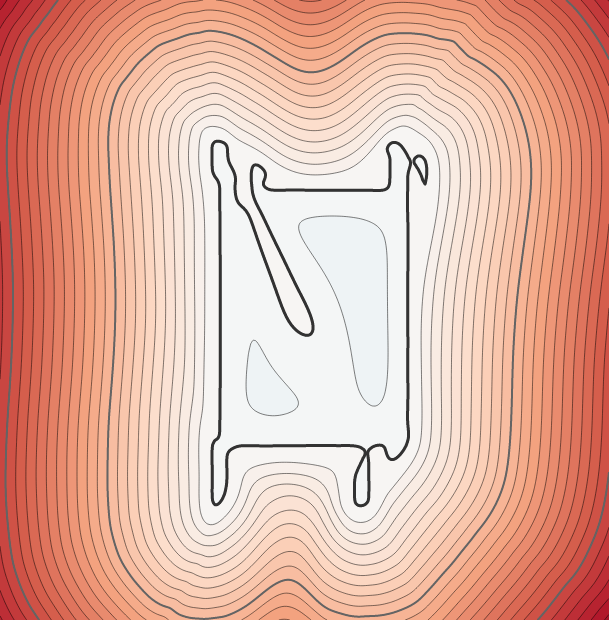
\includegraphics[width=0.11\textwidth]{figures/phase-boundary-exp/3D/cabinet-b0f329dc43af0fbd4da5feafe6f1c8fc-10.0.png} & 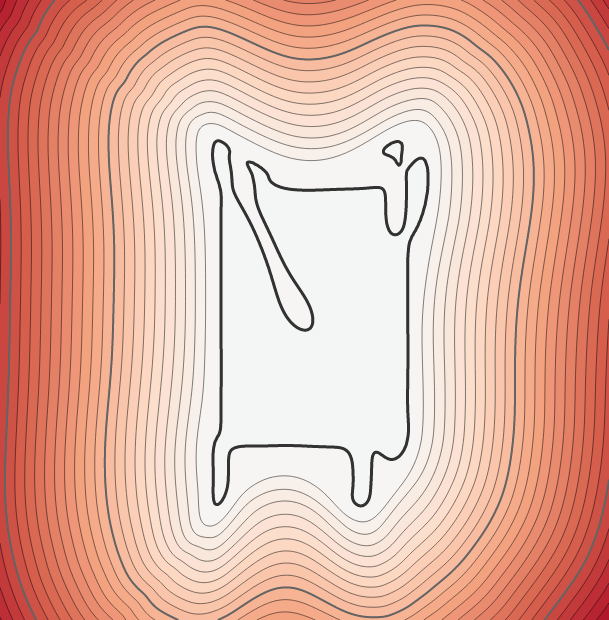
\includegraphics[width=0.11\textwidth]{figures/phase-boundary-exp/3D/cabinet-b0f329dc43af0fbd4da5feafe6f1c8fc-20.0.png} \\
        GT mesh & $w_b = 0.1$ & $w_b = 0.2$ & $w_b = 0.3$ & $w_b = 0.5$ & $w_b = 1.0$ & $w_b = 5.0$ & $w_b = 10.0$ & $w_b = 20.0$ \\
        \toprule
        IoU & 0.0000 & 0.0046 & 0.0387 & 0.1177 & 0.3106 & 0.9742 & 0.9638 & 0.9020 \\
        Chamfer & 0.2056 & 0.2055 & 0.1749 & 0.1441 & 0.0935 & 0.0060 & 0.0065 & 0.0089 \\
        Hausdorff & 0.4905 & 0.4909 & 0.4395 & 0.3855 & 0.3094 & 0.0518 & 0.0545 & 0.0651 \\
        RMSE & 0.8656 & 0.8263 & 0.7944 & 0.7505 & 0.6588 & 0.4578 & 0.4275 & 0.4041 \\
        MAE & 0.8468 & 0.8108 & 0.7769 & 0.7292 & 0.6339 & 0.4004 & 0.3528 & 0.3182 \\
        SMAPE & 1.5123 & 1.5100 & 1.4956 & 1.4608 & 1.3912 & 1.1019 & 0.9778 & 1.0324 \\
        \bottomrule
    \end{tabular}
    \caption{Comparison of PHASE results on a 3D cabinet with different $w_b$ values. SDF values are visualized only on a 2D plane. The color scale is the same as in \Cref{fig:phase-boundary-weight}.}
    \label{fig:phase-boundary-weight-3d}
\end{figure*}

\begin{figure*}[t]
    \setlength{\tabcolsep}{2pt}
    \centering
    \begin{tabular}{cccccccccc}
    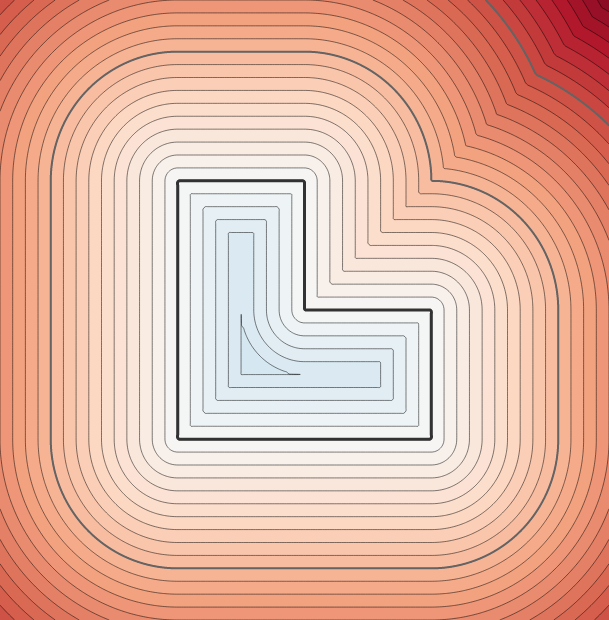
\includegraphics[width=0.09\textwidth]{figures/phase-boundary-exp/2D/L-gt.png} & 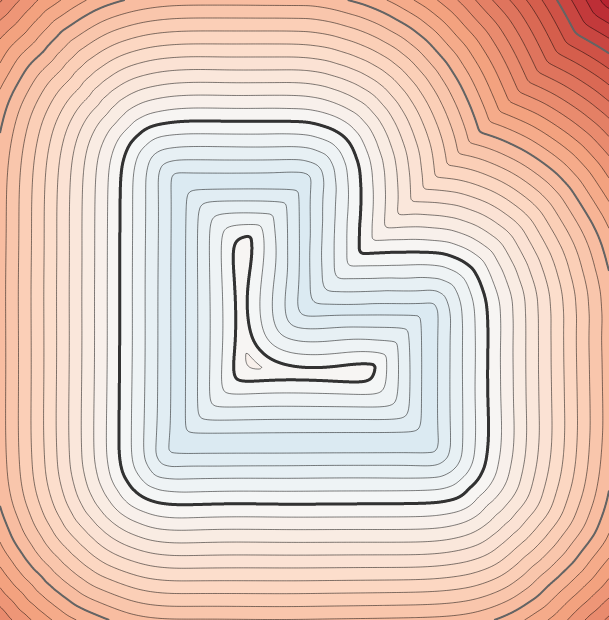
\includegraphics[width=0.09\textwidth]{figures/phase-boundary-exp/2D/L-0.1.png} & 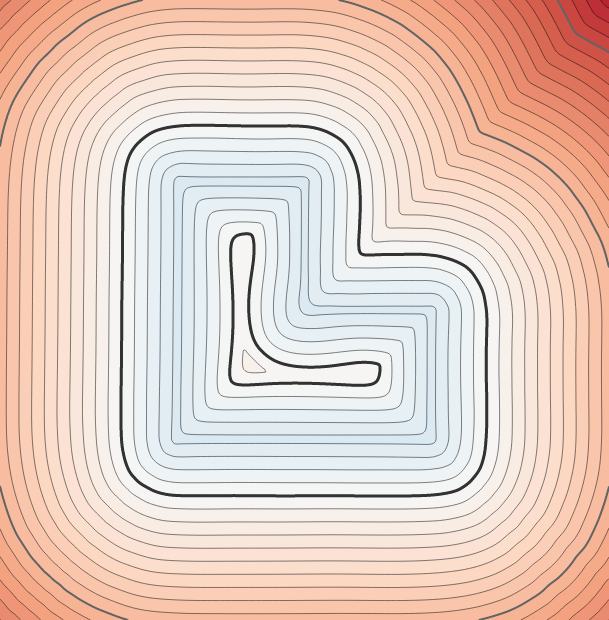
\includegraphics[width=0.09\textwidth]{figures/phase-boundary-exp/2D/L-0.2.png} & 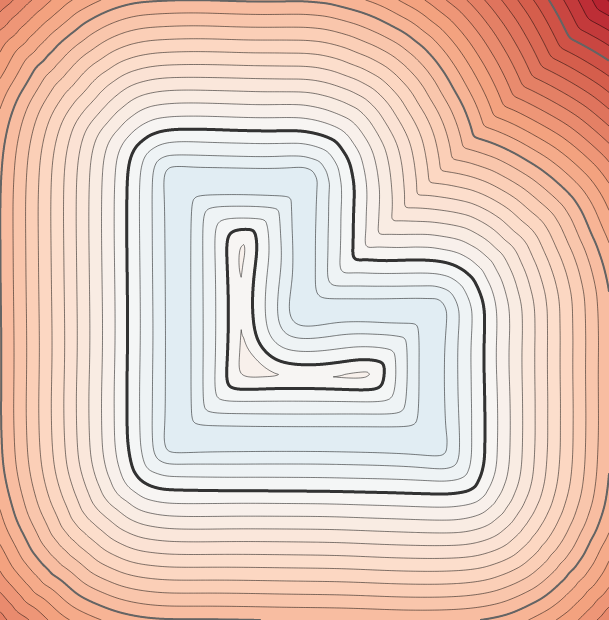
\includegraphics[width=0.09\textwidth]{figures/phase-boundary-exp/2D/L-0.3.png} & 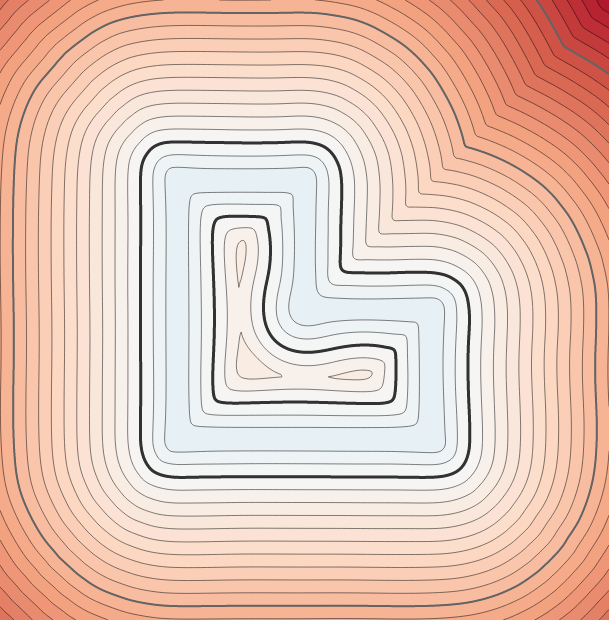
\includegraphics[width=0.09\textwidth]{figures/phase-boundary-exp/2D/L-0.5.png} & 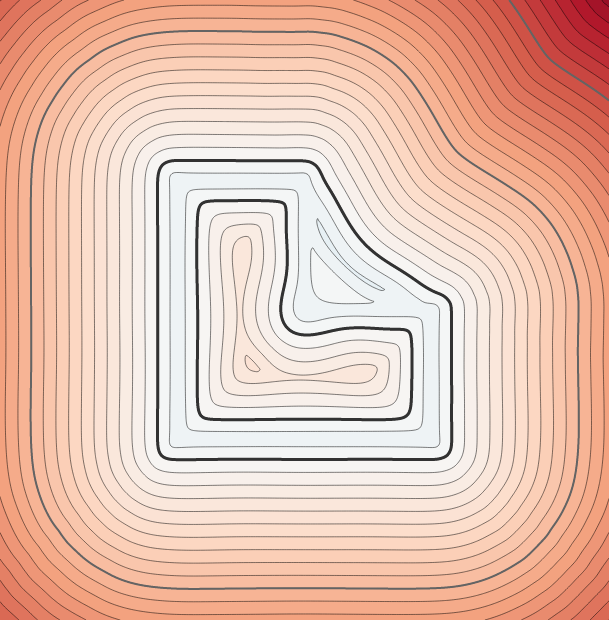
\includegraphics[width=0.09\textwidth]{figures/phase-boundary-exp/2D/L-1.0.png} & 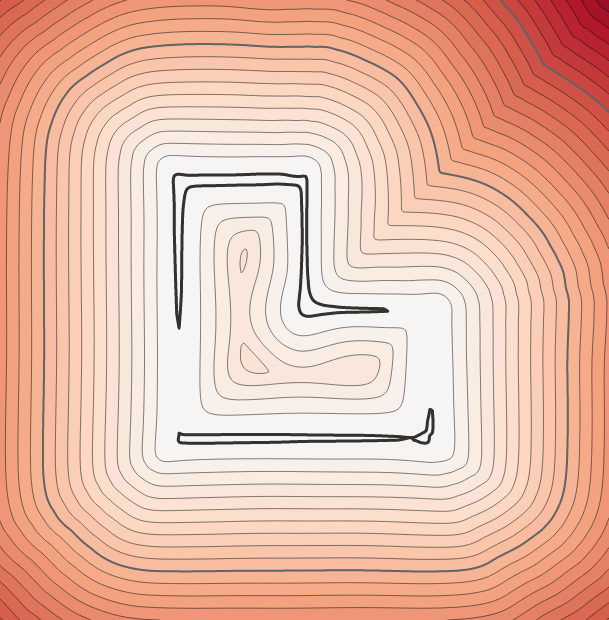
\includegraphics[width=0.09\textwidth]{figures/phase-boundary-exp/2D/L-2.0.png} & 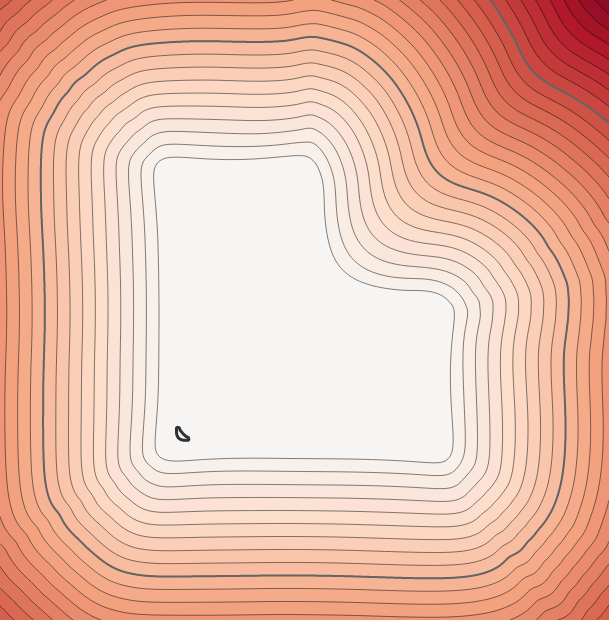
\includegraphics[width=0.09\textwidth]{figures/phase-boundary-exp/2D/L-5.0.png} & 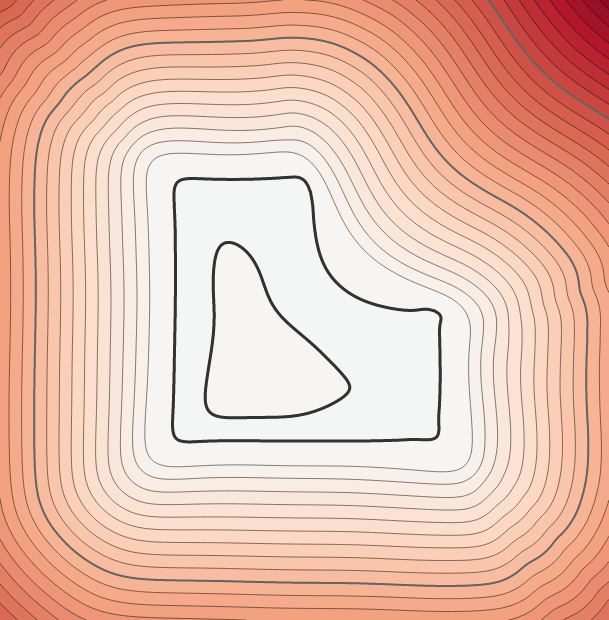
\includegraphics[width=0.09\textwidth]{figures/phase-boundary-exp/2D/L-10.0.png} & 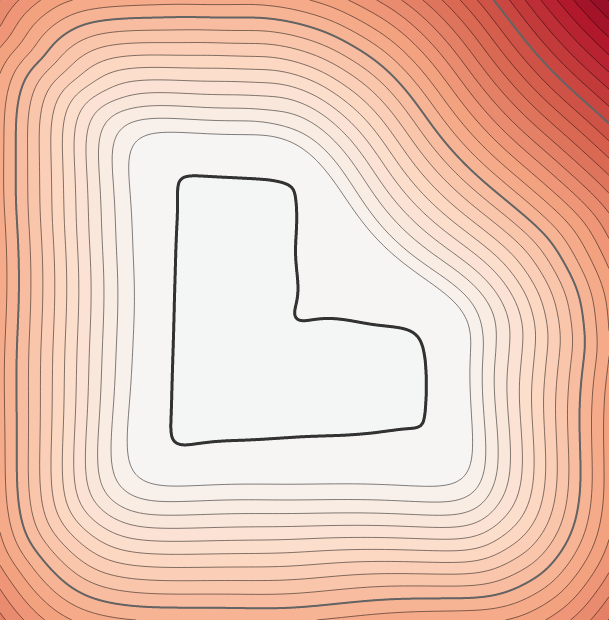
\includegraphics[width=0.09\textwidth]{figures/phase-boundary-exp/2D/L-20.0.png} \\
    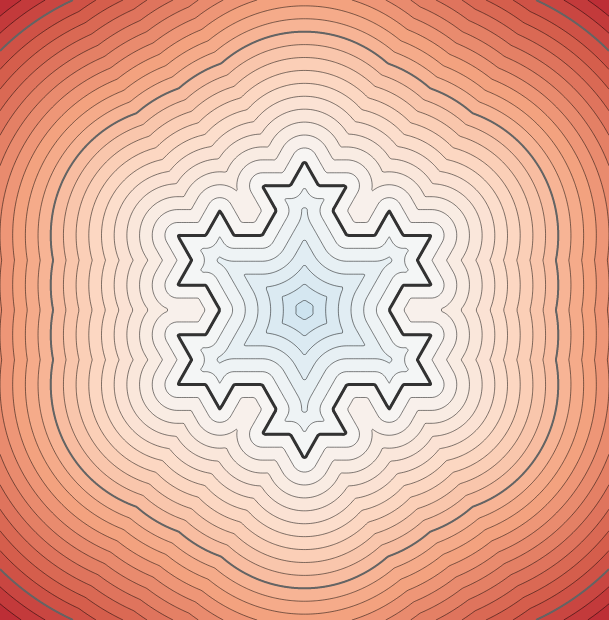
\includegraphics[width=0.09\textwidth]{figures/phase-boundary-exp/2D/snowflake-gt.png} & 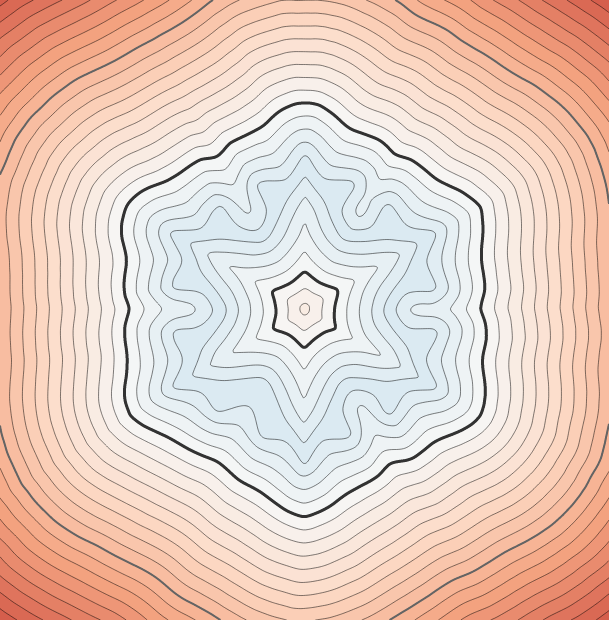
\includegraphics[width=0.09\textwidth]{figures/phase-boundary-exp/2D/snowflake-0.1.png} & 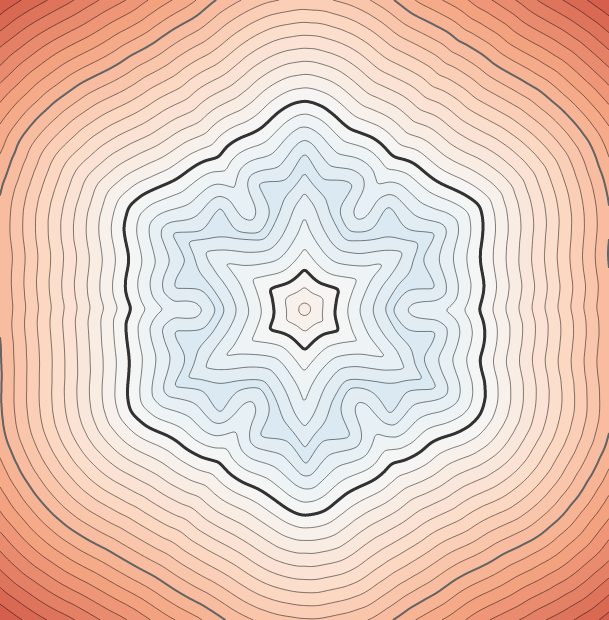
\includegraphics[width=0.09\textwidth]{figures/phase-boundary-exp/2D/snowflake-0.2.png} & 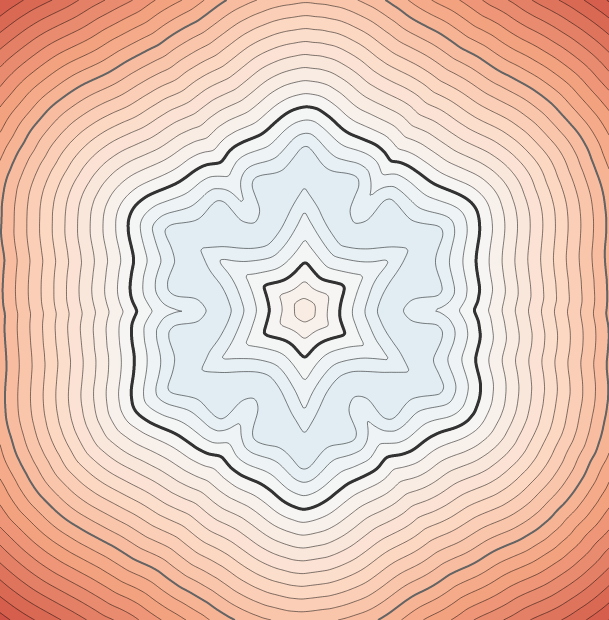
\includegraphics[width=0.09\textwidth]{figures/phase-boundary-exp/2D/snowflake-0.3.png} & 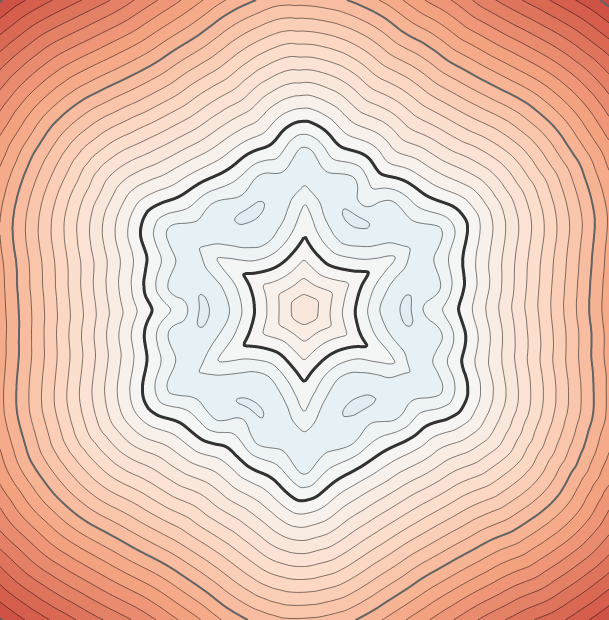
\includegraphics[width=0.09\textwidth]{figures/phase-boundary-exp/2D/snowflake-0.5.png} & 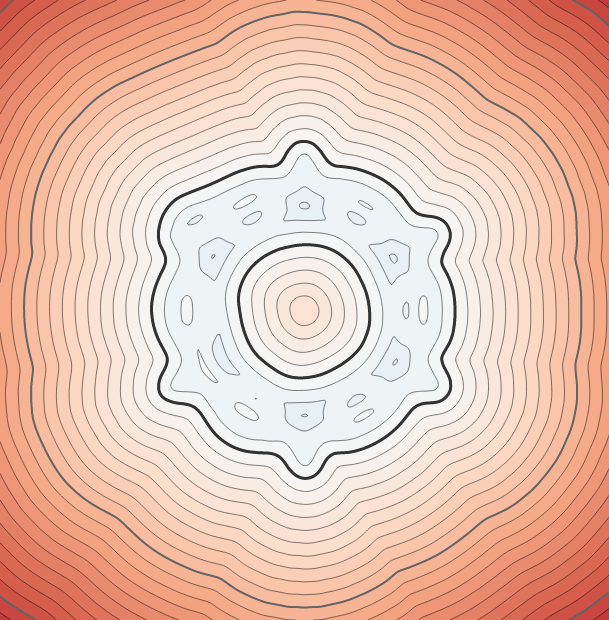
\includegraphics[width=0.09\textwidth]{figures/phase-boundary-exp/2D/snowflake-1.0.png} & 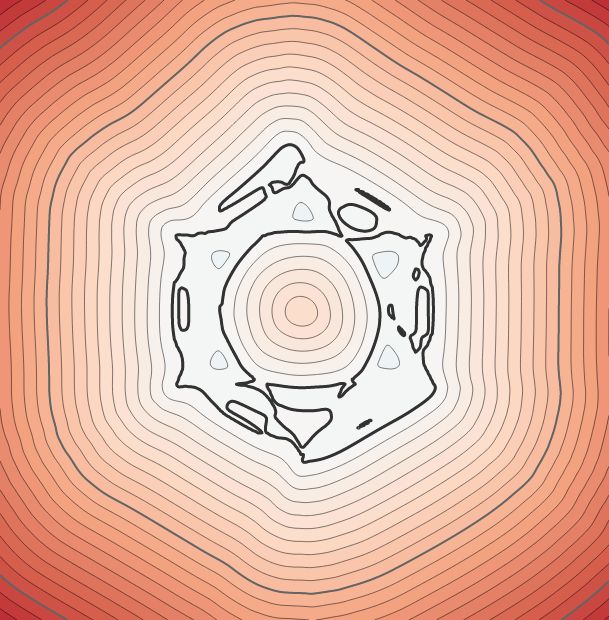
\includegraphics[width=0.09\textwidth]{figures/phase-boundary-exp/2D/snowflake-2.0.png} & 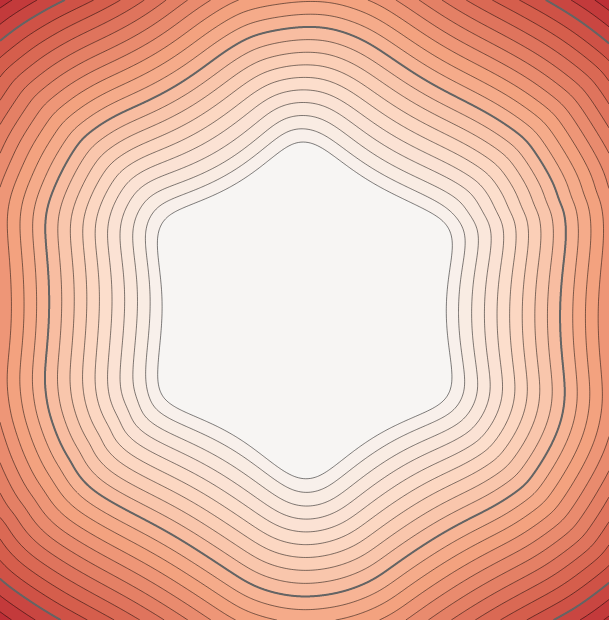
\includegraphics[width=0.09\textwidth]{figures/phase-boundary-exp/2D/snowflake-5.0.png} & 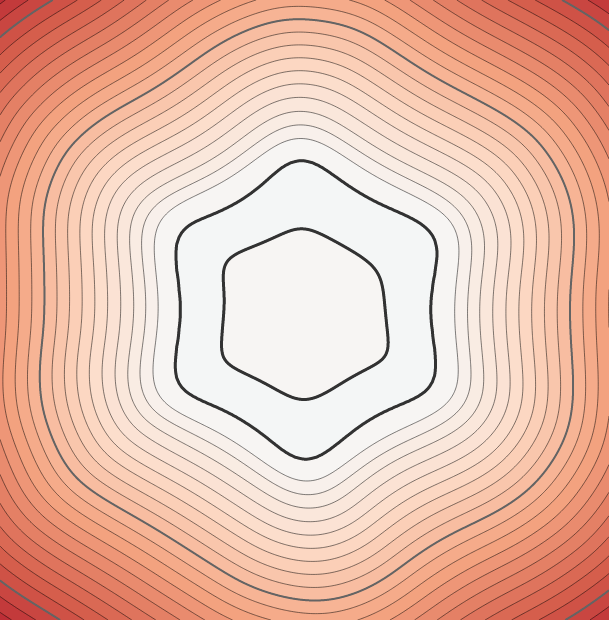
\includegraphics[width=0.09\textwidth]{figures/phase-boundary-exp/2D/snowflake-10.0.png} & 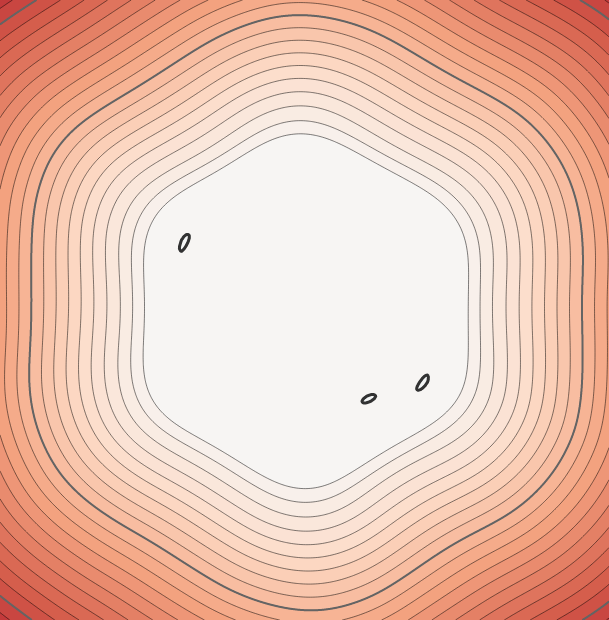
\includegraphics[width=0.09\textwidth]{figures/phase-boundary-exp/2D/snowflake-20.0.png} \\
    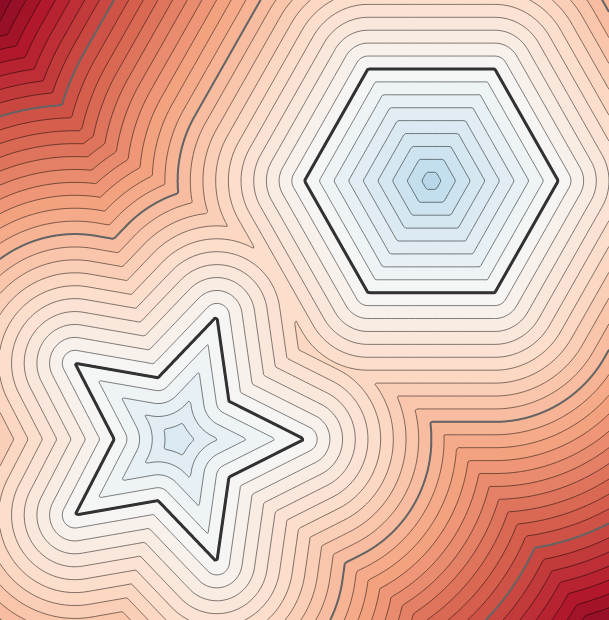
\includegraphics[width=0.09\textwidth]{figures/phase-boundary-exp/2D/starhex-gt.png} & 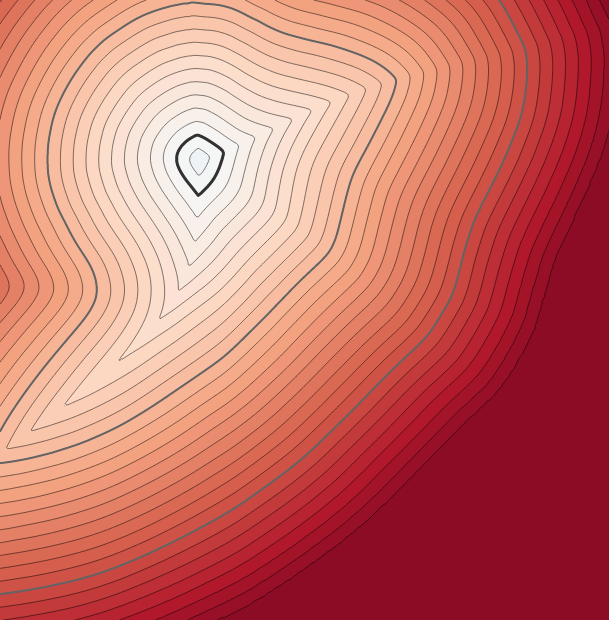
\includegraphics[width=0.09\textwidth]{figures/phase-boundary-exp/2D/starhex-0.1.png} & 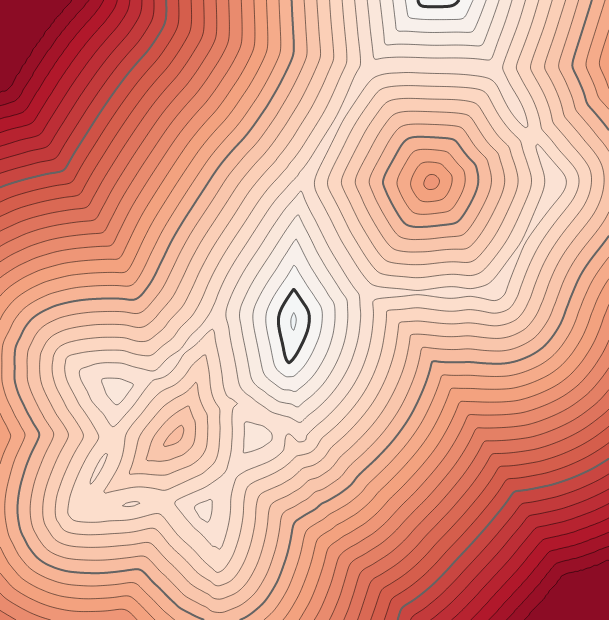
\includegraphics[width=0.09\textwidth]{figures/phase-boundary-exp/2D/starhex-0.2.png} & 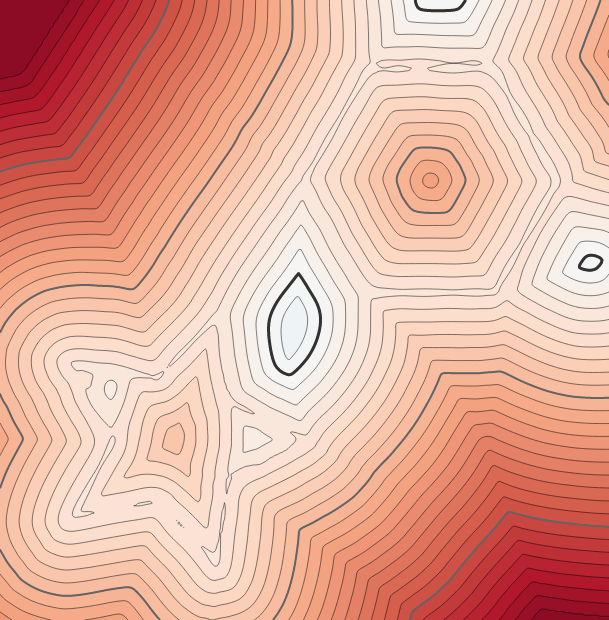
\includegraphics[width=0.09\textwidth]{figures/phase-boundary-exp/2D/starhex-0.3.png} & 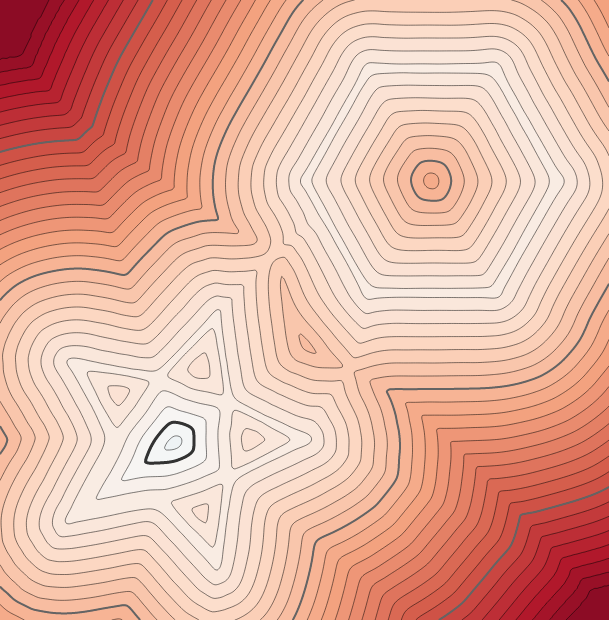
\includegraphics[width=0.09\textwidth]{figures/phase-boundary-exp/2D/starhex-0.5.png} & 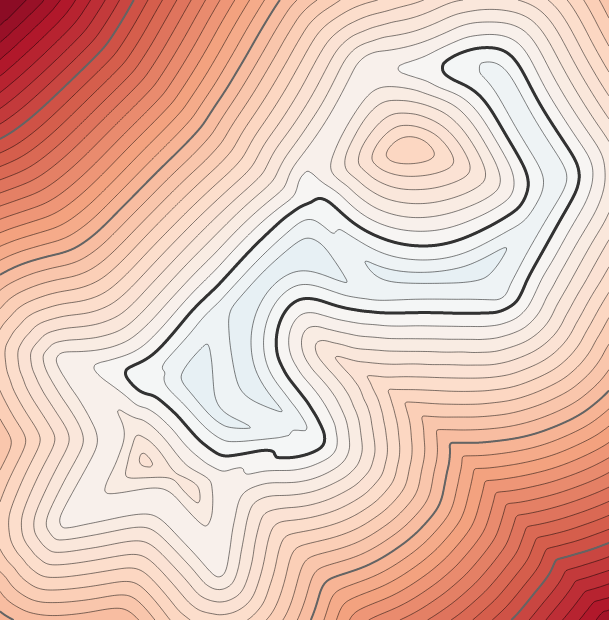
\includegraphics[width=0.09\textwidth]{figures/phase-boundary-exp/2D/starhex-1.0.png} & 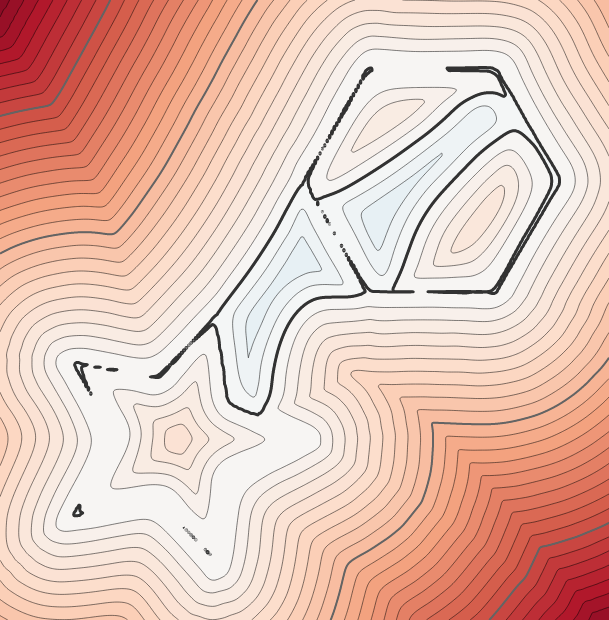
\includegraphics[width=0.09\textwidth]{figures/phase-boundary-exp/2D/starhex-2.0.png} & 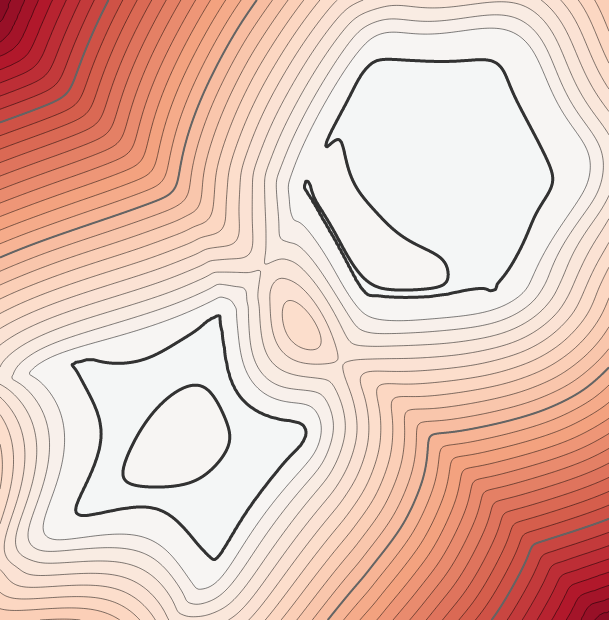
\includegraphics[width=0.09\textwidth]{figures/phase-boundary-exp/2D/starhex-5.0.png} & 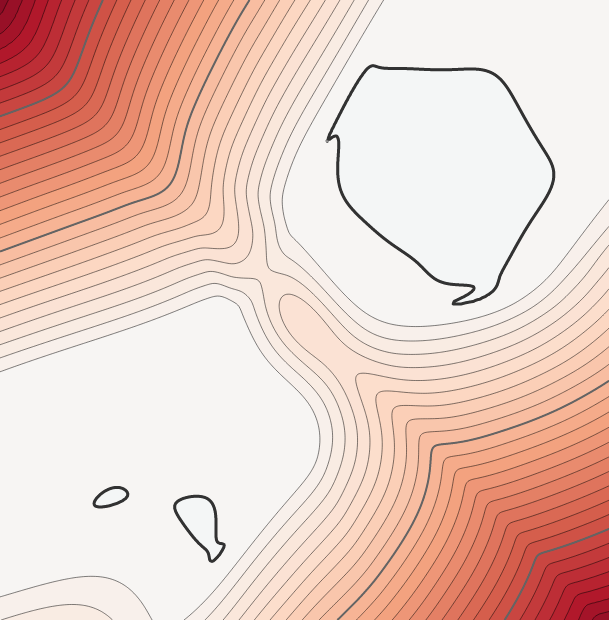
\includegraphics[width=0.09\textwidth]{figures/phase-boundary-exp/2D/starhex-10.0.png} & 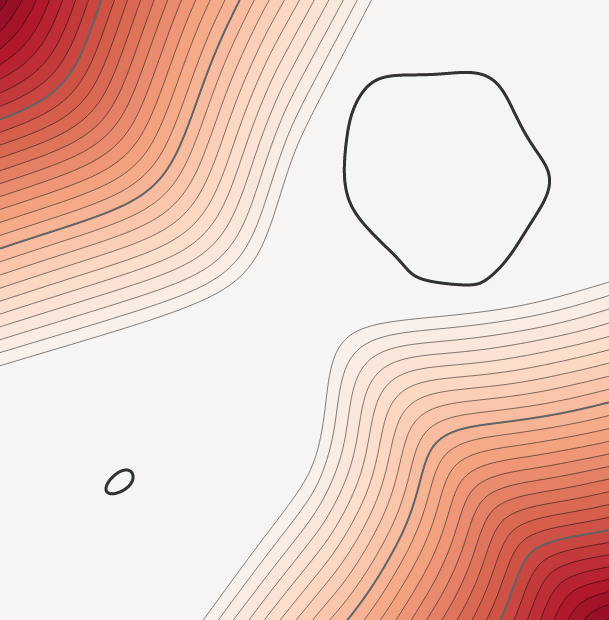
\includegraphics[width=0.09\textwidth]{figures/phase-boundary-exp/2D/starhex-20.0.png} \\
    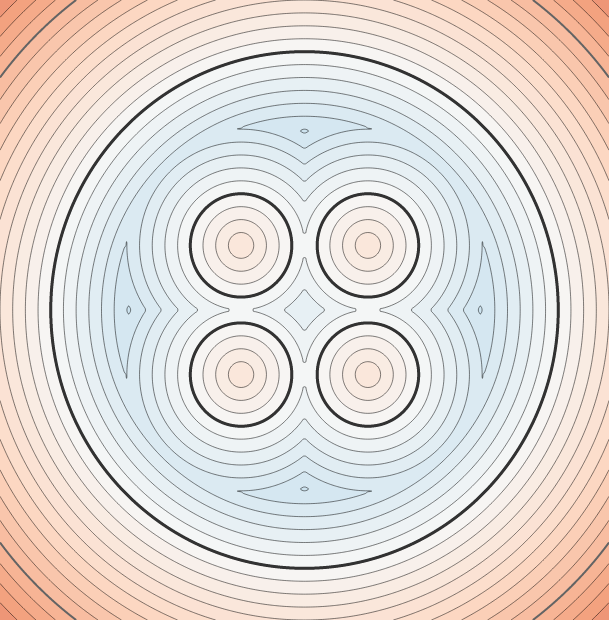
\includegraphics[width=0.09\textwidth]{figures/phase-boundary-exp/2D/button-gt.png} & \includegraphics[width=0.09\textwidth]{figures/phase-boundary-exp/2D/button-0.1.png} & \includegraphics[width=0.09\textwidth]{figures/phase-boundary-exp/2D/button-0.2.png} & \includegraphics[width=0.09\textwidth]{figures/phase-boundary-exp/2D/button-0.3.png} & \includegraphics[width=0.09\textwidth]{figures/phase-boundary-exp/2D/button-0.5.png} & \includegraphics[width=0.09\textwidth]{figures/phase-boundary-exp/2D/button-1.0.png} & \includegraphics[width=0.09\textwidth]{figures/phase-boundary-exp/2D/button-2.0.png} & \includegraphics[width=0.09\textwidth]{figures/phase-boundary-exp/2D/button-5.0.png} & \includegraphics[width=0.09\textwidth]{figures/phase-boundary-exp/2D/button-10.0.png} & \includegraphics[width=0.09\textwidth]{figures/phase-boundary-exp/2D/button-20.0.png} \\
    \includegraphics[width=0.09\textwidth]{figures/phase-boundary-exp/2D/target-gt.png} & \includegraphics[width=0.09\textwidth]{figures/phase-boundary-exp/2D/target-0.1.png} & \includegraphics[width=0.09\textwidth]{figures/phase-boundary-exp/2D/target-0.2.png} & \includegraphics[width=0.09\textwidth]{figures/phase-boundary-exp/2D/target-0.3.png} & \includegraphics[width=0.09\textwidth]{figures/phase-boundary-exp/2D/target-0.5.png} & \includegraphics[width=0.09\textwidth]{figures/phase-boundary-exp/2D/target-1.0.png} & \includegraphics[width=0.09\textwidth]{figures/phase-boundary-exp/2D/target-2.0.png} & \includegraphics[width=0.09\textwidth]{figures/phase-boundary-exp/2D/target-5.0.png} & \includegraphics[width=0.09\textwidth]{figures/phase-boundary-exp/2D/target-10.0.png} & \includegraphics[width=0.09\textwidth]{figures/phase-boundary-exp/2D/target-20.0.png} \\
    \includegraphics[width=0.09\textwidth]{figures/phase-boundary-exp/2D/bearing-gt.png} & \includegraphics[width=0.09\textwidth]{figures/phase-boundary-exp/2D/bearing-0.1.png} & \includegraphics[width=0.09\textwidth]{figures/phase-boundary-exp/2D/bearing-0.2.png} & \includegraphics[width=0.09\textwidth]{figures/phase-boundary-exp/2D/bearing-0.3.png} & \includegraphics[width=0.09\textwidth]{figures/phase-boundary-exp/2D/bearing-0.5.png} & \includegraphics[width=0.09\textwidth]{figures/phase-boundary-exp/2D/bearing-1.0.png} & \includegraphics[width=0.09\textwidth]{figures/phase-boundary-exp/2D/bearing-2.0.png} & \includegraphics[width=0.09\textwidth]{figures/phase-boundary-exp/2D/bearing-5.0.png} & \includegraphics[width=0.09\textwidth]{figures/phase-boundary-exp/2D/bearing-10.0.png} & \includegraphics[width=0.09\textwidth]{figures/phase-boundary-exp/2D/bearing-20.0.png} \\
    \includegraphics[width=0.09\textwidth]{figures/phase-boundary-exp/2D/snake-gt.png} & \includegraphics[width=0.09\textwidth]{figures/phase-boundary-exp/2D/snake-0.1.png} & \includegraphics[width=0.09\textwidth]{figures/phase-boundary-exp/2D/snake-0.2.png} & \includegraphics[width=0.09\textwidth]{figures/phase-boundary-exp/2D/snake-0.3.png} & \includegraphics[width=0.09\textwidth]{figures/phase-boundary-exp/2D/snake-0.5.png} & \includegraphics[width=0.09\textwidth]{figures/phase-boundary-exp/2D/snake-1.0.png} & \includegraphics[width=0.09\textwidth]{figures/phase-boundary-exp/2D/snake-2.0.png} & \includegraphics[width=0.09\textwidth]{figures/phase-boundary-exp/2D/snake-5.0.png} & \includegraphics[width=0.09\textwidth]{figures/phase-boundary-exp/2D/snake-10.0.png} & \includegraphics[width=0.09\textwidth]{figures/phase-boundary-exp/2D/snake-20.0.png} \\
    \includegraphics[width=0.09\textwidth]{figures/phase-boundary-exp/2D/seaurchin-gt.png} & \includegraphics[width=0.09\textwidth]{figures/phase-boundary-exp/2D/seaurchin-0.1.png} & \includegraphics[width=0.09\textwidth]{figures/phase-boundary-exp/2D/seaurchin-0.2.png} & \includegraphics[width=0.09\textwidth]{figures/phase-boundary-exp/2D/seaurchin-0.3.png} & \includegraphics[width=0.09\textwidth]{figures/phase-boundary-exp/2D/seaurchin-0.5.png} & \includegraphics[width=0.09\textwidth]{figures/phase-boundary-exp/2D/seaurchin-1.0.png} & \includegraphics[width=0.09\textwidth]{figures/phase-boundary-exp/2D/seaurchin-2.0.png} & \includegraphics[width=0.09\textwidth]{figures/phase-boundary-exp/2D/seaurchin-5.0.png} & \includegraphics[width=0.09\textwidth]{figures/phase-boundary-exp/2D/seaurchin-10.0.png} & \includegraphics[width=0.09\textwidth]{figures/phase-boundary-exp/2D/seaurchin-20.0.png} \\
    \includegraphics[width=0.09\textwidth]{figures/phase-boundary-exp/2D/peace-gt.png} & \includegraphics[width=0.09\textwidth]{figures/phase-boundary-exp/2D/peace-0.1.png} & \includegraphics[width=0.09\textwidth]{figures/phase-boundary-exp/2D/peace-0.2.png} & \includegraphics[width=0.09\textwidth]{figures/phase-boundary-exp/2D/peace-0.3.png} & \includegraphics[width=0.09\textwidth]{figures/phase-boundary-exp/2D/peace-0.5.png} & \includegraphics[width=0.09\textwidth]{figures/phase-boundary-exp/2D/peace-1.0.png} & \includegraphics[width=0.09\textwidth]{figures/phase-boundary-exp/2D/peace-2.0.png} & \includegraphics[width=0.09\textwidth]{figures/phase-boundary-exp/2D/peace-5.0.png} & \includegraphics[width=0.09\textwidth]{figures/phase-boundary-exp/2D/peace-10.0.png} & \includegraphics[width=0.09\textwidth]{figures/phase-boundary-exp/2D/peace-20.0.png} \\
    \includegraphics[width=0.09\textwidth]{figures/phase-boundary-exp/2D/boomerangs-gt.png} & \includegraphics[width=0.09\textwidth]{figures/phase-boundary-exp/2D/boomerangs-0.1.png} & \includegraphics[width=0.09\textwidth]{figures/phase-boundary-exp/2D/boomerangs-0.2.png} & \includegraphics[width=0.09\textwidth]{figures/phase-boundary-exp/2D/boomerangs-0.3.png} & \includegraphics[width=0.09\textwidth]{figures/phase-boundary-exp/2D/boomerangs-0.5.png} & \includegraphics[width=0.09\textwidth]{figures/phase-boundary-exp/2D/boomerangs-1.0.png} & \includegraphics[width=0.09\textwidth]{figures/phase-boundary-exp/2D/boomerangs-2.0.png} & \includegraphics[width=0.09\textwidth]{figures/phase-boundary-exp/2D/boomerangs-5.0.png} & \includegraphics[width=0.09\textwidth]{figures/phase-boundary-exp/2D/boomerangs-10.0.png} & \includegraphics[width=0.09\textwidth]{figures/phase-boundary-exp/2D/boomerangs-20.0.png} \\
    \includegraphics[width=0.09\textwidth]{figures/phase-boundary-exp/2D/fragments-gt.png} & \includegraphics[width=0.09\textwidth]{figures/phase-boundary-exp/2D/fragments-0.1.png} & \includegraphics[width=0.09\textwidth]{figures/phase-boundary-exp/2D/fragments-0.2.png} & \includegraphics[width=0.09\textwidth]{figures/phase-boundary-exp/2D/fragments-0.3.png} & \includegraphics[width=0.09\textwidth]{figures/phase-boundary-exp/2D/fragments-0.5.png} & \includegraphics[width=0.09\textwidth]{figures/phase-boundary-exp/2D/fragments-1.0.png} & \includegraphics[width=0.09\textwidth]{figures/phase-boundary-exp/2D/fragments-2.0.png} & \includegraphics[width=0.09\textwidth]{figures/phase-boundary-exp/2D/fragments-5.0.png} & \includegraphics[width=0.09\textwidth]{figures/phase-boundary-exp/2D/fragments-10.0.png} & \includegraphics[width=0.09\textwidth]{figures/phase-boundary-exp/2D/fragments-20.0.png} \\
    \includegraphics[width=0.09\textwidth]{figures/phase-boundary-exp/2D/house-gt.png} & \includegraphics[width=0.09\textwidth]{figures/phase-boundary-exp/2D/house-0.1.png} & \includegraphics[width=0.09\textwidth]{figures/phase-boundary-exp/2D/house-0.2.png} & \includegraphics[width=0.09\textwidth]{figures/phase-boundary-exp/2D/house-0.3.png} & \includegraphics[width=0.09\textwidth]{figures/phase-boundary-exp/2D/house-0.5.png} & \includegraphics[width=0.09\textwidth]{figures/phase-boundary-exp/2D/house-1.0.png} & \includegraphics[width=0.09\textwidth]{figures/phase-boundary-exp/2D/house-2.0.png} & \includegraphics[width=0.09\textwidth]{figures/phase-boundary-exp/2D/house-5.0.png} & \includegraphics[width=0.09\textwidth]{figures/phase-boundary-exp/2D/house-10.0.png} & \includegraphics[width=0.09\textwidth]{figures/phase-boundary-exp/2D/house-20.0.png} \\
        
    GT & $w_b = 0.1$ & $w_b = 0.2$ & $w_b = 0.3$ & $w_b = 0.5$ & $w_b = 1.0$ & $w_b = 2.0$ & $w_b = 5.0$ & $w_b = 10.0$ & $w_b = 20.0$ \\[1ex]
    \end{tabular}
    \caption{Comparison of PHASE results with different $w_b$ values on the rest of the 2D dataset. The color scale is the same as in \Cref{fig:phase-boundary-weight}.}
    \label{fig:phase-boundary-weight-more}
\end{figure*}